\documentclass[10pt]{article}

%%%%    FORMATTING    %%%%
\usepackage{url}
\usepackage[utf8]{inputenc}
\usepackage{amsmath}
\usepackage{amssymb}
\usepackage{lineno}
%\usepackage{wasysym}
\usepackage[dvipsnames]{xcolor}
\usepackage[version=4]{mhchem}
\usepackage{verbatim}
\usepackage{graphicx}
\usepackage[export]{adjustbox}
\usepackage[margin=1in]{geometry}
\usepackage[titletoc, title]{appendix}
\usepackage{hyperref}
\hypersetup{
    colorlinks = true,
    citecolor = red,
    linkcolor = blue,
    urlcolor = blue,
}
%For code in appendix
\usepackage{listings}
\usepackage{color}
\definecolor{mygreen}{rgb}{0,0.6,0}
\definecolor{mygray}{rgb}{0.5,0.5,0.5}
\definecolor{mymauve}{rgb}{0.58,0,0.82}
\lstset{ %
  backgroundcolor=\color{white},   % choose the background color
  basicstyle=\footnotesize,        % size of fonts used for the code
  breaklines=true,                 % automatic line breaking only at whitespace
  captionpos=b,                    % sets the caption-position to bottom
  commentstyle=\color{mygreen},    % comment style
  escapeinside={\%*}{*)},          % if you want to add LaTeX within your code
  keywordstyle=\color{blue},       % keyword style
  stringstyle=\color{mymauve},     % string literal style
  frame = tb,
  numbers = left
}




\title{nEXO OD FLUKA Simulations Manual}
\author{Regan Ross}

%%%%    BEGIN DOCUMENT    %%%
\begin{document}

%%%%    Title Page    %%%
\begin{titlepage}
    \maketitle
    \vspace{4cm}
    \centering
    % \includegraphics*[scale=0.5, frame]{./figs/muons_det.png}
\end{titlepage}

\begin{abstract}
    This document is intented to provide insight into the functioning of the nEXO FLUKA simulations and justifications for choices made in their design. Further, this work should provide a near comprehensive baseline for anyone willing to replicate similar cosmogenic studies for the nEXO collaboration, or even another. FLUKA can be a daunting software to work with given it is written in FORTRAN77, has sparse documentation, and whose source code, without a specific licence, is veiled to the user. However, this proprietary simulation program is fast and rich with built-in features that have been used extensively for decades \cite{FLUKA1}, \cite{FLUKA2}. Moreover, it is particularly useful for the case of studying cosmogenic muons at several hundred GeV energies and their secondaries \cite{gratta_muons_to_neutrons} \cite{KamLand_Zen}. This document will provide an overview and explanation of the FLUKA features enabled for the specific nEXO Outer Detector (OD) case and an overview of the additional user routines, scripts, and containerization procedures that are all ancilliary to the base simulations (but required to run the simulations on the SDF cluster and perform the more in-depth analyses required by our questions).  All references hereafter to the FLUKA manual refer to \cite{FLUKA_Manual}.


\end{abstract}

\vspace{1.5cm}
\listoffigures

\newpage
\tableofcontents

\break
%%%%%%%%%%%%%%%%%%%%%%%%%%%%%%%%%%%%%%
%                                   %
%%%%    The FLUKA Input File     %%%%
%                                   %
%%%%%%%%%%%%%%%%%%%%%%%%%%%%%%%%%%%%%%

%\part*{Input to FLUKA}

\section{The nEXO OD Input File}
\paragraph{}
The input file (``.inp'') is exactly as it is named— it is the De facto interface between the user and the FLUKA binaries. It contains, among other things, the entire physical configuration of the media through which the particles are transported, the defining characteristics of the impinging beam (for simple sources), options for enabling particular physical processes, definitions of materials, and cards to deploy default FLUKA scoring methods. It is a human-readable ascii file with a very specific format. Each input card in the input file must not contain more than 8 fields each of which has a character limit. This is due (presumably) to constraints in the early development of FLUKA. Programmed in FORTRAN77 which imposes constrains on the length of statements which, in the early days, were written into computers (with very little memory) using paper punch cards. Now, this formatting is an annoying anachronism but it probably does still keep the program slim and fast. Generally though, a user need not worry about writing the input file directly, as there is a great GUI interface to FLUKA called \href{https://fluka.cern/documentation/examples/flair}{\textit{Flair}} which, by the way, is open source and contains all the possible input options \cite{Flair}. The next section will overview the specific components of the nEXO OD input file and the functions they serve. 

\paragraph{}
It is expected that the user interfaces with the input files via \href{https://fluka.cern/documentation/examples/flair}{\textit{Flair}} as this is probably the easiest way. Errors in the configuration will be unambiguously shown, and it is hard to mess up the format of the input file this way.

\subsection{Geometry}

\paragraph{}
Arguably the most important parts of the input file are the cards defining the configuration space— namely the detector and media with respect to the cartesian coordinate system. In FLUKA this is known as the \textit{geometry}. The geometry section of the input card is demarcated by \textbf{GEOBEGIN} and \textbf{GEOEND} cards. Between these two cards are first, cards for various \textit{bodies} which are basic 2D and 3D geometric surfaces and second, cards for \textit{regions} whose bounds are defined by combinations of geometric \textit{bodies}. For instance, a triplet of bodies could be a cylinder whose axis lies on the $z$-axis, and two planes lying parallel the $x-y$ plane at different $z$s. A region defined by these bodies could be the 3D cylindrical volume made by the cylinder body capped off on either end by the two planes. This is exactly the type of region representing the nEXO OD and the nEXO TPC. 

\begin{figure}[h]
    \begin{center}
    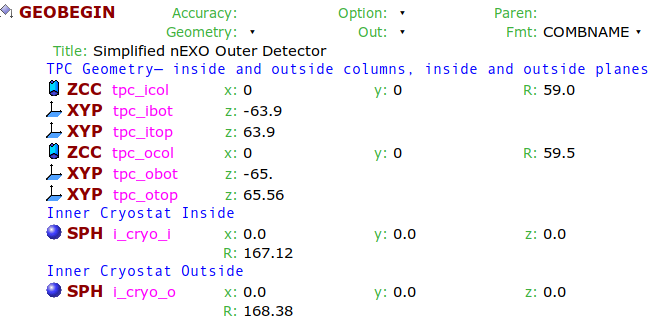
\includegraphics[scale=0.5]{figures/geometry_1.png}
    \caption{An example of the geometry body declarations in the input file}
    \label{fig:geometry1}
    \end{center}
\end{figure}

\paragraph{}
Figure \ref{fig:geometry1} shows the first part of the geometry declarations in the nEXO input file. We see the first card is the \textbf{GEOBEGIN} with the argument \textit{fmt} set to COMBNAME. This tells the FLUKA binaries how to read in the following geometry cards. This is not particularly important. This seems to be the default mode. Text in \textcolor{blue}{blue} indicates a comment (equivalent to a FORTRAN77 comment in the input file) and body variable names are in \textcolor{magenta}{pink} and are limited to lengths of 8 characters. The names or types of cards are fully capitalized and in \textcolor{Maroon}{maroon}. The argument names for each card are written in \textcolor{ForestGreen}{green} and the arguments follow with an 8 character length limit. These colour conventions hold for every other type of input card. Each card can have many arguments, but generally, not all are necessary. In the geometry body cards however, each argument is provided as these arguments are all necessary to uniquely define their respective geometric body. For instance, there is a body called \textcolor{magenta}{i\_cryo\_i} defined with a \textcolor{Maroon}{SPH} card. The name is intented to be shorthand for ``inner cryostat inside'' and, being a sphere, requires a radius and three coordinates for its location in space. There are many choices for bodies in FLUKA, each of which fairly simple to define.

\paragraph{}
Regions, as previously discussed, are created with logical combinations of bodies. Imagine the bodies defining surfaces in 3D, and the regions being the volumes they surround. Following the set of cards defining the bodies, there is an \textbf{END} card, then the region cards as shown in figure \ref{fig:geometry2}, finally there is the \textbf{GEOEND} card. Each region must be assigned \textbf{one} material— we'll get to material assignments later. For example, the region inside the nEXO OD that is full of water would be defined by the OD inside body minus the outer cryostat outside body leaving the configuration of a cylinder with a spherical hole in its volume— the entirety of this region is to be water. 

\begin{figure}[h]
    \begin{center}
    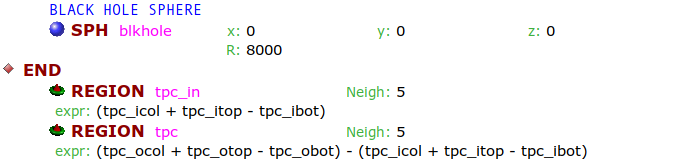
\includegraphics[scale=0.5]{figures/geometry_2.png}
    \caption{An example of the geometry region declarations in the input file}
    \label{fig:geometry2}
    \end{center}
\end{figure}

\paragraph{}
Looking at figure \ref{fig:geometry2}, we see the final body declaration followed by the first few region declarations in the nEXO input file. The final body here is important— each FLUKA configuration defines its physical boundaries by assigning material \textit{blackhole} to its outermost surface- hence the name of the sphere. The first region we have defined is \textcolor{magenta}{tpc\_in} will be the inside of the TPC cylinder— the part filled with liquid xenon. While no number is assigned by the user to the region, FLUKA assigns it number 1 as it is the first defined- this will be important later. The construction of the region is in the \textcolor{ForestGreen}{expr} argument given by ``(tpc\_icol $+$ tpc\_itop $-$ tpc\_ibot)''. We first have \textit{tpc\_icol} which is the inside cylinder (along $z$) of the TPC which alone is unbound and spans the entire $z$-axis. To the cylinder we add \textit{tpc\_itop} (xy-plane) which sets the upper bound, and subtract \textit{tpc\_ibot} (xy-plane) which sets the lower bound. This process is similar for all other region declarations. Unfortunately, one may not reference regions by name in region expressions, only bodies; hence the following region declaration of the \textcolor{magenta}{tpc} which is intended to be the material composing the TPC. The \textcolor{ForestGreen}{Neigh} argument is an integer which defines ``neighbourhoods'' relating regions to each other. This can perhaps be deployed for larger, more complex geometries but given the simplicity of the nEXO OD geometry and the lack of thorough documentation of this feature, it has been set to the default value of 5 for each region. Once more, the \textbf{GEOEND} card (not shown) brings us to the end of the geometry card section.

\subsubsection{The Chosen Configuration}
\paragraph{}
The simulations performed here deployed a simplified geometry of nEXO. There were no PMTs included, no complicated internal structure and no contoured cavernous room around the detector. It is simply a large stainless steel cylinder surrounded by norite rock \cite{olivia_scallon} and full of water containing the inner and outer cryostats and the copper TPC filled with liquid Xenon-136. That's it. The muons are propogated through at least 15m of rock before reaching the detector, and the rock surrounding the OD laterally is 20m, and below it, 5m. Where possible, the measurements for the configuration were taken from the ``nEXO Preliminary Design Report'' except for the size of the OD which has been adjusted to meet the more recent specification.

\begin{figure}[h]
    \begin{center}
    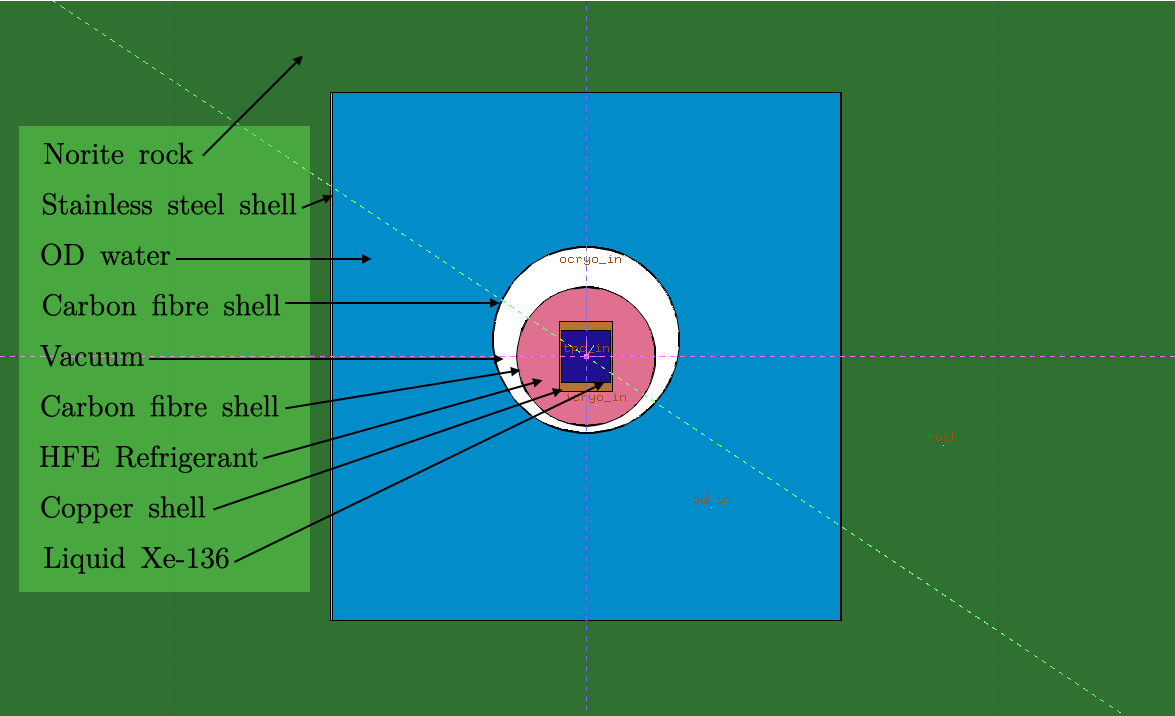
\includegraphics[scale=0.3]{figures/geometry_3.png}
    \caption{A 2D projection of the nEXO geometry used in the FLUKA simulations}
    \label{fig:geometry3}
    \end{center}
\end{figure}


\subsection{Media}
\label{sec:Media}
\paragraph{}
After \textit{geometry} the most natural section to discuss in the input card is the \textit{Media} section. In this section, materials are defined if they aren't in the FLUKA default material database and they're assigned to regions. There are four main types of cards in this section: \textcolor{Maroon}{MATERIAL}, \textcolor{Maroon}{COMPOUND}, \textcolor{Maroon}{ASSIGNMA}, and \textcolor{Maroon}{LOW-MAT}. 

\begin{figure}[h]
    \begin{center}
    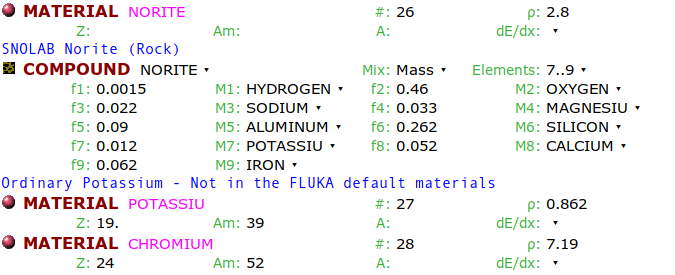
\includegraphics[scale=0.5]{figures/media_1.png}
    \caption{A subset of the media section in the input file}
    \label{fig:media1}
    \end{center}
\end{figure}

\paragraph{}
First, referring to figure \ref{fig:media1} and describe the first card in the media section. It is a \textcolor{Maroon}{MATERIAL} card with variable name \textcolor{magenta}{NORITE}. This card declares a new material called \textcolor{magenta}{NORITE} which is given a density, and a user-chosen material number for later reference \footnote{The numbers for user-defined materials can't start at 1, they proceed from the last number of the native FLUKA materials list (25)}. Norite rock is an abundant rock around the Sudbury basin. It is a mixture of various elements and must therefore be defined with the subsequent \textcolor{magenta}{COMPOUND} card. The arguments for this card are the component materials of the compound and their respective fractions by mass, volume, or atom abundance. These arguments should be very clear, the odd one out is \textcolor{ForestGreen}{Elements} which simply allows for the resizing of the compound card to accomodate more or fewer elements. The following cards, \textcolor{magenta}{POTASSIU} and \textcolor{magenta}{CHROMIUM} are necessary to define as they are not in the default FLUKA materials list. Given that these are elemental, we must provide the arguments of atomic number (\textcolor{ForestGreen}{Z}), the atomic mass (\textcolor{ForestGreen}{Am}) in g/mol, and the atomic mass number (\textcolor{ForestGreen}{A}) which is assumed to be the most abundant for the given (\textcolor{ForestGreen}{Z}) if left unspecified. Of course \textcolor{ForestGreen}{$\rho$} is the density, and \textcolor{ForestGreen}{$dE/dx$} allows to select another material to use for the case of ionization— we do not use this feature.

\paragraph{}
Once all the materials are defined they are then assigned to regions with the \textcolor{Maroon}{ASSIGNMA} cards. This card a list of arguments including the material to be assigned and the regions it will be assigned to. One of these cards can assign a material to several regions, however, the regions had to have been declared in some regular order for this to work for multiple regions. That is, a user might wish to have every region from the first to last of N regions to be full of water. In this case, the card would have arguments \textcolor{ForestGreen}{Reg:} $=$ 1 and \textcolor{ForestGreen}{to Reg:} $= N$. Alternatively, a user can assign a material to every $k^{\text{th}}$ region in the range $[1,N]$ by setting \textcolor{ForestGreen}{Step:} $=$ 3. This seems like a strange and uncomfortable way to do things because any modification to the region declarations can totally offset the material assignments. Nevertheless, it is how it works. In the ``nEXO\_OD.inp'' input file, each region is assigned a material separately and by name. This issue ought not occur.

\subsubsection{Specific Materials}
\paragraph{}
Now that the media input options have been discussed, we will overview some of the materials used in the ``nEXO\_OD.inp'' input file as these may not be an exact representation of the material structure of nEXO. First, the rock surrounding the geometry is of a particular variety that is very common around SNOLAB: norite \cite{SNOLAB_dose}. Its composition is shown in the table below. Then, another compound used in the configuration is HFE, the refrigerant in the inner cryostat whose composition is shown in the table below. 

\begin{center}
    \label{tab:norite}
    \begin{tabular}[h]{|c|c|}
        \hline
        \multicolumn{2}{|c|}{Norite $\rho = 2.894 $ g/cm$^3$} \\
        \hline
        \hline
        Element & Atomic Composition (\%) \\
        \hline
        O & 46.0 \\
        Si & 26.2 \\
        Al & 9.0 \\
        Fe & 6.2 \\
        Ca & 5.2 \\
        Mg & 3.3 \\
        Na & 2.2 \\
        K & 1.2 \\
        Ti & 0.5 \\
        H & 0.15 \\
        Mn & 0.1 \\
        C & 0.04 \\
        \hline
    \end{tabular}
    \quad
    \label{tab:HFE}
    \begin{tabular}[h]{|c|c|}
        \hline
        \multicolumn{2}{|c|}{HFE $\rho \approx 1.5 $ g/ml} \\
        \hline
        \hline
        Element & Atomic Composition (\%) \\
        \hline
        F & 46.6 \\
        C & 26.7 \\
        H & 20.0 \\
        O & 6.7 \\
        \hline
    \end{tabular}
\end{center}


\subsection{Physics and Particle Transport}

\paragraph{}
By default, FLUKA transports neutrons down to $1 \times 10^{-5}$ eV or ``thermal energies''. Some other physics processes have to be enabled explicitly using various FLUKA cards. For instance, photo-nuclear events between muons and nuclei are not enabled by default. Figure \ref{fig:physics1} below shows the set of physics cards currently used in the nEXO input file. In all cards with the arguments ``\textcolor{ForestGreen}{Mat:}'' and ``\textcolor{ForestGreen}{to Mat:}'', the respective arguments are ``HYDROGEN'' and ``@LASTMAT''. This simply means that these processes are enabled in all materials from the first to last FLUKA material in the file. Namely, hydrogen has FLUKA material number 1, and the materials used in section \ref{sec:Media} extend to some arbitrary highest integer— @LASTMAT.

\begin{figure}[h]
    \begin{center}
    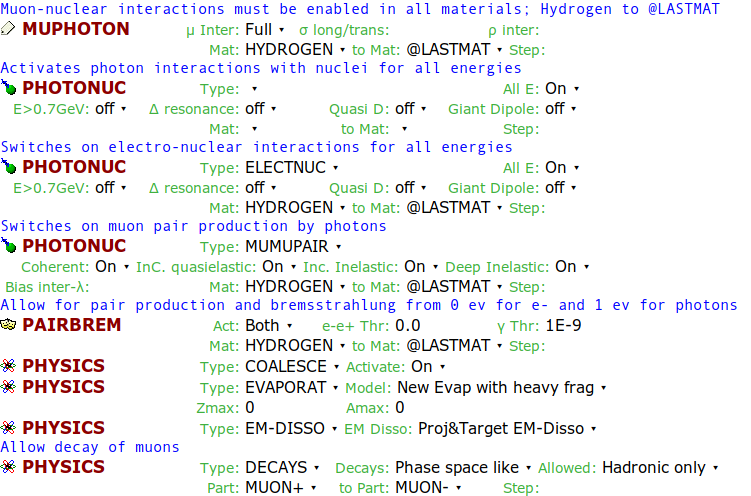
\includegraphics[scale=0.5]{figures/physics.png}
    \caption{The set of physics cards in the nEXO input file}
    \label{fig:physics1}
    \end{center}
\end{figure}

\paragraph{\textcolor{Maroon}{MUPHOTON}}
This is used to enable muon photonuclear interactions and to allow for the production of all secondary hadrons by muons. In this card, the arguments not provided are reserved for code development and not in use.

\paragraph{\textcolor{Maroon}{PHOTONUC}}
These cards are used to activate gamma interactions with nuclei. The first in the series requires only the ``\textcolor{ForestGreen}{All E}'' argument to be ON to enable photonuclear interactions over all energies in FLUKA. The second two \textcolor{Maroon}{PHOTONUC} cards are used to activate electronuclear interactions and muon-muon pair production respectively.

\paragraph{\textcolor{Maroon}{PAIRBREM}}
This card controls simulation of pair production and bremsstrahlung by high-energy muons, charged hadrons and light ions (up to alpha's). Here, both bremsstrahlung and pair production are activated with the electron energy threshold set to 0 which corresponds to the lowest FLUKA limits, and the $\gamma$ threshold set to 1 eV.

\subsection{Scoring}

\paragraph{}
Also within the input file are some scoring options. In FLUKA, the \textit{measurables} are \textit{scored} or synonymously, \textit{estimated}. Nevertheless, the scoring section of the input file contains a few cards activating the builtin scoring features of FLUKA, and another single card that requests the custom scoring from within the ``mgdraw.f'' file.

\begin{figure}[h]
    \begin{center}
    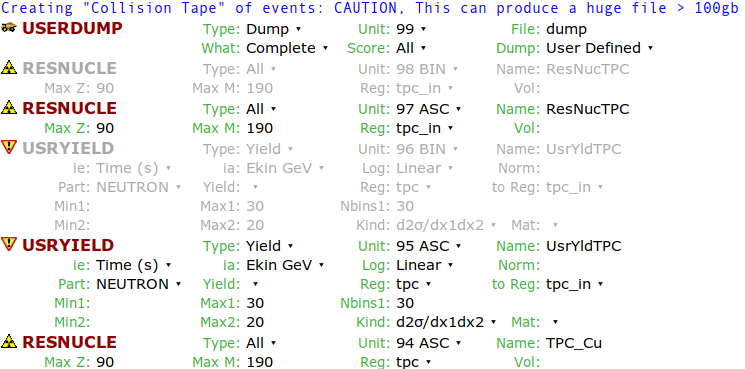
\includegraphics[scale=0.5]{figures/scoring.png}
    \caption{The set of scoring cards in the nEXO input file}
    \label{fig:scoring}
    \end{center}
\end{figure}

\paragraph{}
In figure \ref{fig:scoring} there is the entirety of the scoring section in the input card. The \textcolor{Maroon}{USERDUMP} card specifies that the ``mgdraw.f'' routine gets called to enable the customized scoring therein. However, one has to be careful as the default ``mgdraw.f'' file can save \textbf{much} more data than is necessary resulting in files exceeding tens of gigabytes in size— hence the \textcolor{Blue}{comment} above the card.

\paragraph{}
The \textcolor{Maroon}{RESNUCLE} cards tell FLUKA to print out ascii (human-readable) files which contain the counts of residual nuclei in a given region. Seen here we have cards for the TPC liquid xenon and also the copper TPC shell. 

\paragraph{}
Data from the other scoring cards are not currently used but they can be used to score differential fluence (with respect to energy, time, etc...). In essence all one needs for the nEXO scoring are the residual nuclei scoring cards for activation, and the USERDUMP which sends the data to the custom routine that takes care of the rest of the neutron data.


%\part*{The Muon Source User Routine}

\section{Muon Source}

\begin{figure}[h]
    \begin{center}
    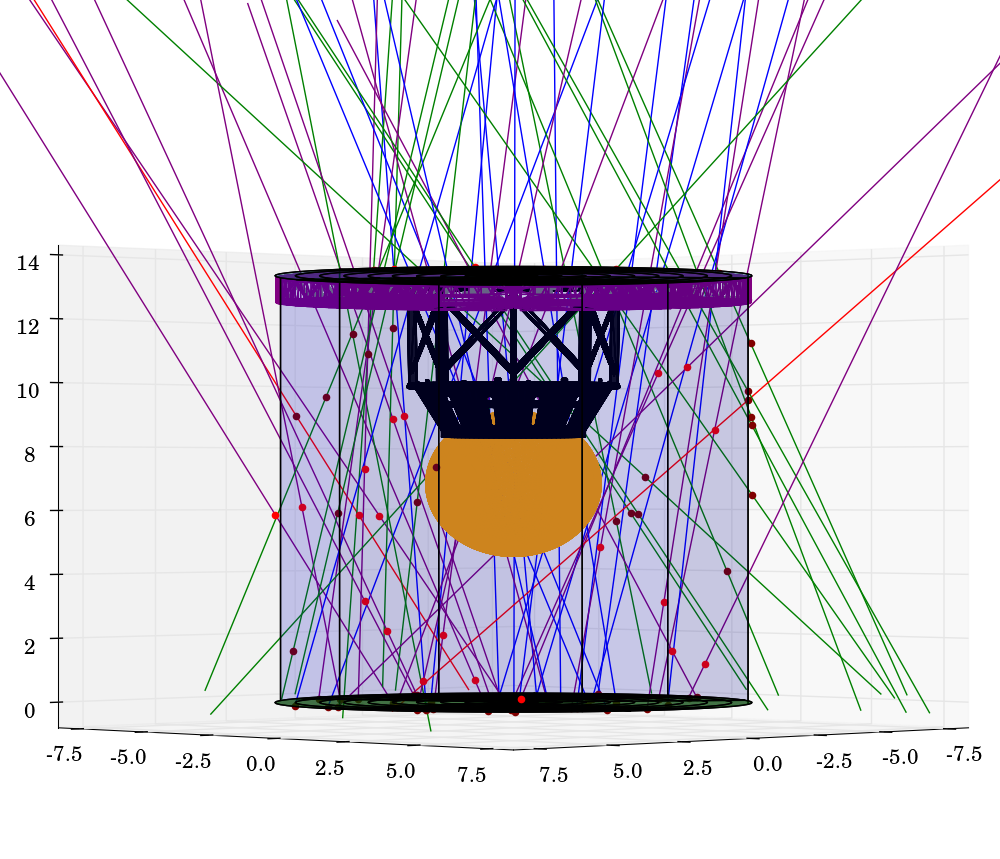
\includegraphics[scale=0.3]{figures/muons_1.png}
    \caption{A visualization of muons passing through a more sophisticated nEXO geometry}
    \label{fig:muons_1}
    \end{center}
\end{figure}

\paragraph{}
In FLUKA, one may define a beam-like source using the built-in \textcolor{Maroon}{BEAM} cards. However, if one wishes to simulate a more novel or complex series of source particles, a different user routine can do the trick. In the FLUKA literature and on the forums, this more complex source file is called ``source\_newgen.f''. In the simulation files here, it is called ``muon\_from\_file.f'' as this makes more sense. This user routine comes with a set of built-in functions allowing a sophisticated user to sample energies from various functions (Maxwell-Boltzmann for instance) and sample various initial positions. In our case, however, we only make use of a pair of features— the \textit{real} source generation is done with a more easily readable and modifiable set of python functions. To learn about how the muons are simulated, please see \cite{rross_muon_technote}.

\paragraph{}
In ``muon\_from\_file.f'' particles are read from a phase-space file (we'll get to that) and passed to FLUKA where they are propogated through the configuration and scored as requested. This is done using the built in routine ``read\_phase\_space\_file''. In this user routine, a file argument is provided pointing to the list of muons (called a phase space file). This is kept in the ``sim\_files'' directory and created with each run using the ``run\_simulation.py'' script (for now). The files are created externally using the muon\_functions.py module in the ``sim\_tools'' directory. Basically, the file contains a list of muons with attributes listed as comma-separated values in the following order:

\[
    \begin{matrix}
        \text{Particle No.} & \text{Energy  [GeV]} & X_0 \text{ [m]} & Y_0 \text{ [m]}& Z_0 \text{ [m]}& \cos(x) & \cos(y) & -\cos(z) & \text{Weight}
    \end{matrix}
\]

or equivalently in FLUKA language:

\[
    \begin{matrix}
        \text{JTRACK} & \text{ETRACK} & \text{XSCO} & \text{YSCO} & \text{ZSCO} & \text{CXTRCK} & \text{CYTRCK} & \text{CZTRCK} & \text{WTRACK}
    \end{matrix}
\]

\paragraph{}
The particle number (JTRACK) is either 10 (positive muon) or 11 (negative muon). These variables will be further discussed in the section on customized scoring here: \ref{tab:mgdraw_vars}. 



%\part*{The Scoring User Routine (`mgdraw.f')}

\section{Customized Scoring}

\paragraph{}
While for many general purposes FLUKA comes equipped with adequate features, more particular circumstances may call for probing the particle stack directly. This is done through external user routines that are only deployed when explicitly linked at compile time. For instance, to determine the distances of closest approach for muons that produce neutrons in the TPC region, access to these data is necessary. For the most part, all the features of FLUKA can be accessed with customized code through the ``mgdraw.f'' user routine.

%\part*{Interpreting Output}

\clearpage

\section{Some Results}
\paragraph{}
The primary motivation for these FLUKA simulations was to validate the GEANT4 simulations that had previously been performed to estimate activation due to the cosmogenic muons. Other connections were investigated including the distances of closest approach (impact parameters) of the muons producing neutrons in the vicinity of the nEXO OD. There had been a connection established between the impact parameters and the propensity of a muon to produce neutrons within or entering the OD or the TPC volume; muons with large impact parameters were unlikely to contribute to activation.

\paragraph{}
For the simulations in this work, the impact parameters were calculated upon the random generation of the muons in the external python module. These data, along with all the other muon data, were saved and added to the ``.hdf5'' files after the simulations were performed. The activation data were scored with FLUKA's RESNUCLEi function that counts ``residual nuclei'' in a chosen region. The analyses were entirely performed externally using various python libraries.

\subsection{Activation}

\paragraph{}
The activation was scored for the TPC internal liquid xenon volume and its copper shell. 

\begin{appendices}

\begin{figure}[h]
    \begin{center}
    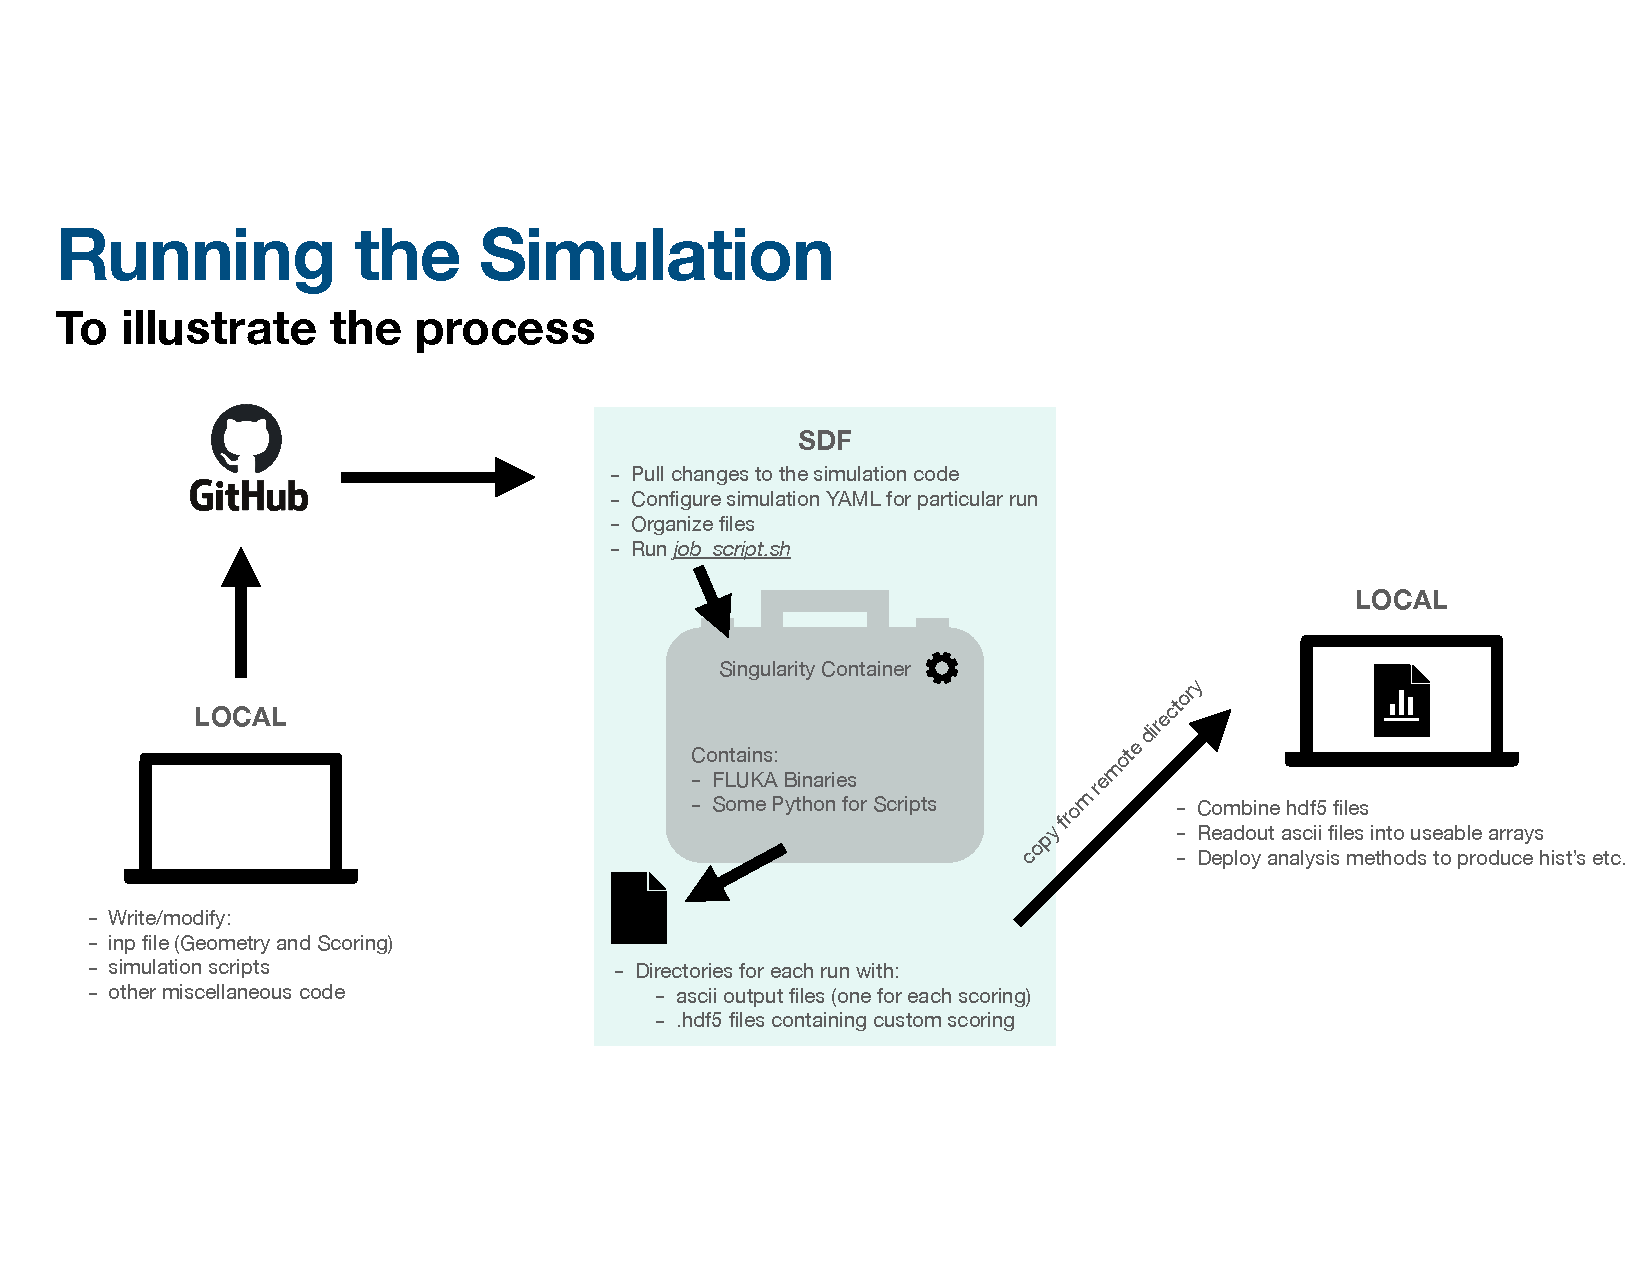
\includegraphics[scale=0.5]{figures/sim_diagram.pdf}
    \caption{A visualization of the remote simulation and development process}
    \label{fig:process1}
    \end{center}
\end{figure}

\section*{Containerization with Singularity}

\paragraph{}
In order to deploy FLUKA on a remote cluster, SDF for instance, it must be packaged up in a \textit{container}. SDF recommends using Singularity which is essentially designed for containerizing software with its dependencies to maximize portability. Naturally, there are a few caveats to containerizing the simulation. The first, rather inconvenient constraint is that Singularity containers must (at the time of writing) be built from within a Linux OS. Therefore, to build a Singularity image using a Mac, one must use a linux VM. This requires, among other pieces, Vagrant which is used to run the Linux virtual machine. There's no use in giving a comprehensive guide to installing Singularity, Vagrant and creating the entire Singularity image here; these softwares are actively being developed and improved. Readers are referred to the Sylabs Singularity documentation: \url{https://docs.sylabs.io/guides/3.11/admin-guide/installation.html#mac}.

\paragraph{}
The definition file ``\begin{tt}.def\end{tt}'' for the Singularity container is in the Github repository. Should the reader wish to reproduce or modify the container, they'll need at minimum a CERN FLUKA licence in order to download the FLUKA binaries and they'll need to be placed in the directory where the container will be created along with any other files and software that cannot be installed separately from within the ``\begin{tt}.def\end{tt}'' file.
\section{Submitting Jobs with SLURM}


\paragraph{}
When running FLUKA simulations on a computing cluster such as SDF, one has to submit \textit{jobs} to be performed. These are the tasks that you are requesting the computer perform; for instance, you may submit a job of simulating 5000 muons in your geometry. The simulations performed here were generally submitted in batches— many jobs at once. Each job would require a node (a CPU) and these would each churn through two-months worth of muons through the OD simultaneously.  The SDF cluster uses SLURM to allocate jobs and thus we will briefly discuss SLURM here as it pertains to running the FLUKA simulations. Following this section is an example of a job submission script used to submit jobs to the SDF cluster.

\paragraph{}
In the following script, the first line tells the interpreter to use \textit{bash} to interpret the uncommented lines. Bear in mind, this script is not run in the conventional way by entering its path into the terminal, but by typing \textit{SBATCH} followed by the path to the script. Now, the next commented (\#) lines beginning with SBATCH are commands read in exclusively by SLURM. These request the specific resources for each node in the array (we're requesting an array of jobs here— see line 14). Each node will have 3 hours and 30 minutes to complete the task before the job will be ended by SLURM (line 13). Then for each one of these nodes, the following bash commands are executed (line 19 onward).

\begin{linenumbers}
\begin{verbatim}
#!/bin/bash

#################################################
#                   SLURM
#################################################

#SBATCH --partition=shared
#SBATCH --job-name=fluka_sims               # a short name for your job
#SBATCH --output=simrun-%A-%a.out           # stdout file
#SBATCH --error=simrun-%A-%a.err            # stderr file
#SBATCH --cpus-per-task=1                   # cpu-cores per task (>1 if multi-threaded tasks)
#SBATCH --mem-per-cpu=10G                   # memory per cpu-core (4G is default)
#SBATCH --time=03:30:00                     # total run time limit (HH:MM:SS)
#SBATCH --array=0-50                        # job array with index values 0, 1, 2, 3, 4

#################################################
#                  Variables
#################################################

output_dir="run"$SLURM_ARRAY_JOB_ID

rand=$RANDOM
path_to_sim='/gpfs/slac/staas/fs1/g/exo/exo_data8/exo_data/users/rross/flukaSims/'
image=$path_to_sim"fluka_nEXO.sif"
job_num=$SLURM_ARRAY_JOB_ID         # An integer number representing this array job submission
task_num=$SLURM_ARRAY_TASK_ID       # An integer within the array range above representing which part of the parallelized run
fluka_path='/usr/local/fluka/bin/'

muon_source=$path_to_sim'muon_from_file.f'
mgdraw=$path_to_sim'mgdraw_neutron_count.f'
input=$path_to_sim'nEXO_OD.inp'

new_muon_source=$path_to_sim'musource'$rand'.f'
new_muon_source_o=$path_to_sim'musource'$rand'.o'
new_mgdraw=$path_to_sim'mgdrw'$rand'.f'
new_mgdraw_o=$path_to_sim'mgdrw'$rand'.o'
new_input=$path_to_sim'input'$rand'.inp'
exe_name=path_to_sim'exe'$rand'.exe'

#################################################
#    REMEMBER: These do not run sequentially.
################################################

mkdir $output_dir
mkdir $output_dir/subrun$SLURM_ARRAY_TASK_ID

#################################################
#         Printing meta data to stdout
################################################

cd $path_to_sim
date
echo "Executing on the machine:" $(hostname) 
echo "System random number used to seed the sim:" $rand
echo "Running Simulation!"
echo ; echo ; echo ; echo "COMPILING JARGON:"
echo

singularity exec -B /gpfs $image python $path_to_sim/run_simulation.py -s $rand

mv *$rand* $output_dir/subrun$SLURM_ARRAY_TASK_ID
mv *.hdf5 $output_dir/
\end{verbatim}
\end{linenumbers}
\section{Running the simulation}

\paragraph{}
Other users of this code may choose to make adjustments to better suit their needs, but for now, this is how the code is generally run. Not every command will be reviewed here, but a general description of the procedure will be provided. 

\begin{figure}[h]
    \begin{center}
    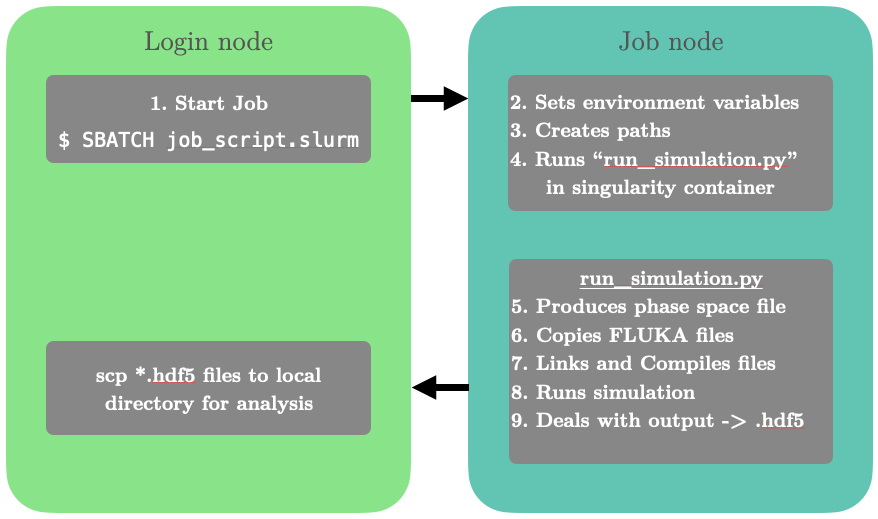
\includegraphics[scale=0.5]{figures/nodes.png}
    \caption{A simple display of what is happening when the code is run}
    \label{fig:running}
    \end{center}
\end{figure}
\section{HDF5 File Structure}

\paragraph{}
It's in the name; HDF5 (hierarchical data format) files have a hierarchy. Within the file there are groups, within the groups there are datasets. Within the datasets there are data. Figure \ref{fig:h5_file} shows the current data format for the h5 output files.

\begin{figure}[h]
    \begin{center}
    \includegraphics[scale=0.2]{figures/fluka_h5_key.png}
    \caption{The structure of the output hdf5 files}
    \label{fig:h5_file}
    \end{center}
\end{figure}

\end{appendices}


% \newpage

% \section*{Acknowledgements}
% \paragraph{}

\bibliographystyle{aip}
\bibliography{manual.bib}

\end{document}